\documentclass[onecolumn, conference]{IEEEtran}
\IEEEoverridecommandlockouts
% The preceding line is only needed to identify funding in the first footnote. If that is unneeded, please comment it out.
\usepackage{cite}
\usepackage{amsmath,amssymb,amsfonts}
\usepackage{algorithmic}
\usepackage{graphicx}
\usepackage{textcomp}
\usepackage{subfigure}
\usepackage{xcolor}
\def\BibTeX{{\rm B\kern-.05em{\sc i\kern-.025em b}\kern-.08em
    T\kern-.1667em\lower.7ex\hbox{E}\kern-.125emX}}
\begin{document}

\title{ADSP Final Project}


\author{
\IEEEauthorblockA{Wang Sifan} \\
\textit{2020231067}
\and
\IEEEauthorblockA{Zheng Yueyang} \\
\textit{2020231112}

}

\maketitle



\section{Scenario 1: Analyze hearing aid array configuration}
\subsection{Desired source located at 0 degrees and Interferer located at 135 degrees}

Fig.~\ref{Beampattern of left two microphones135}, Fig.~\ref{Beampattern of upper two microphones135} and Fig.~\ref{Beampattern of all four microphones135} are the beampatterns in different frequency.  In Fig.~\ref{Beampattern of left two microphones135}, beampatterns in different frequency are almost the same. That's because when we use the left two microphones, \(d=0.01m\) and \(\frac{d}{\lambda}<\frac{1}{2} \) for $f = 500,1000,2000,4000$Hz, which all leads to oversampling. We get the same gain at \(135^{\circ}\) and \(-135^{\circ}\) because \(\cos\theta = \cos(-\theta)\) and this leads to the symmetry. When we use upper two microphones (Fig.~\ref{Beampattern of upper two microphones135}), \(d=0.14m\) and \(\frac{d}{\lambda}=\frac{1}{2} \)  when \(f=2000Hz\). There is an undersamlping when \(f=4000Hz\) which causes the spatial aliasing and a bad performance. We get the same gain at \(135^{\circ}\) and \(45^{\circ}\) because \(\sin\theta = \sin(\pi-\theta)\). When we increase the number of sensors (Fig.~\ref{Beampattern of all four microphones135}), the beampattern has little difference with Fig.~\ref{Beampattern of upper two microphones135}. Since we put the sensors in square, this eliminate the undesired gain from symmetry.

\begin{figure}[htbp]
	\begin{minipage}[b]{0.5\linewidth}
		\centerline{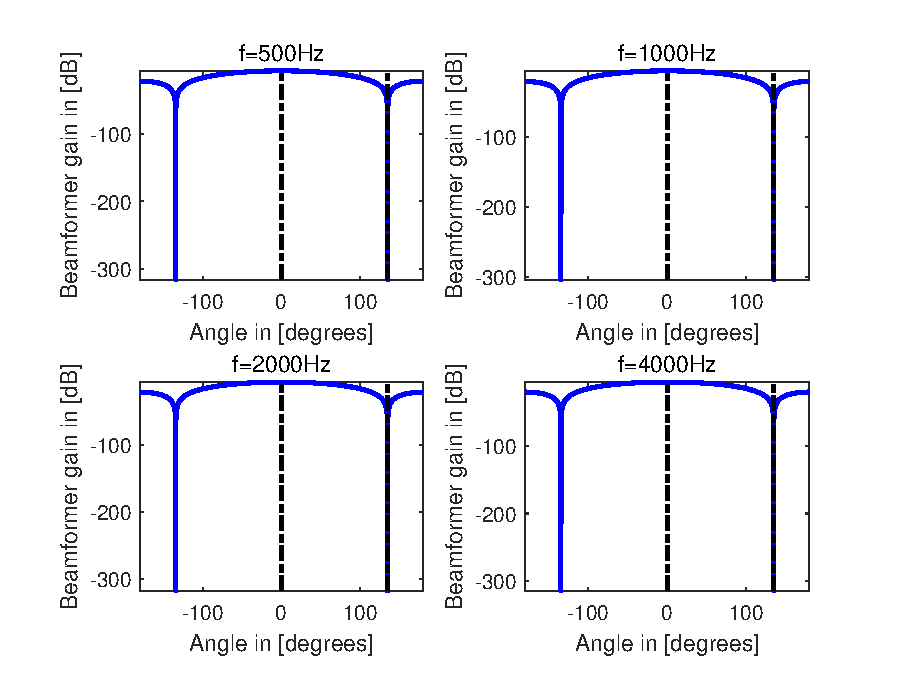
\includegraphics[width=1\textwidth]{img/1_a_1.eps}}
		\caption{Beampattern of left two microphones}
		\label{Beampattern of left two microphones135}
	\end{minipage}
	\hfill
	\begin{minipage}[b]{0.5\linewidth}
		\centerline{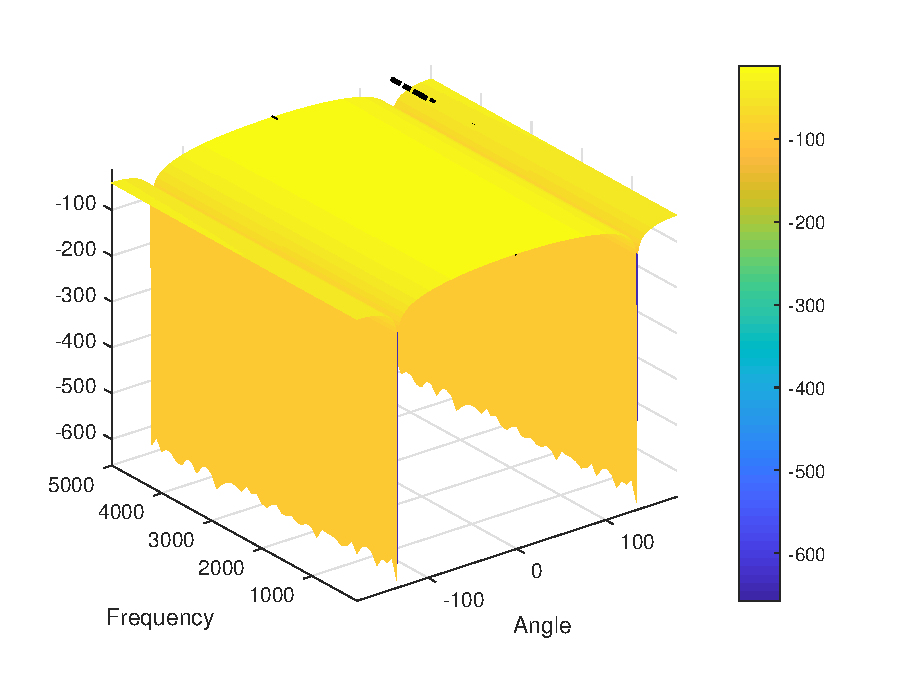
\includegraphics[width=1\textwidth]{img/1_a_1_multi_135.eps}}
		\caption{Multitone beampattern of left two microphones}
		\label{Multitone beampattern of left two microphones135}
	\end{minipage}
\end{figure}

\begin{figure}[htbp]
\begin{minipage}[b]{0.5\linewidth}
	\centerline{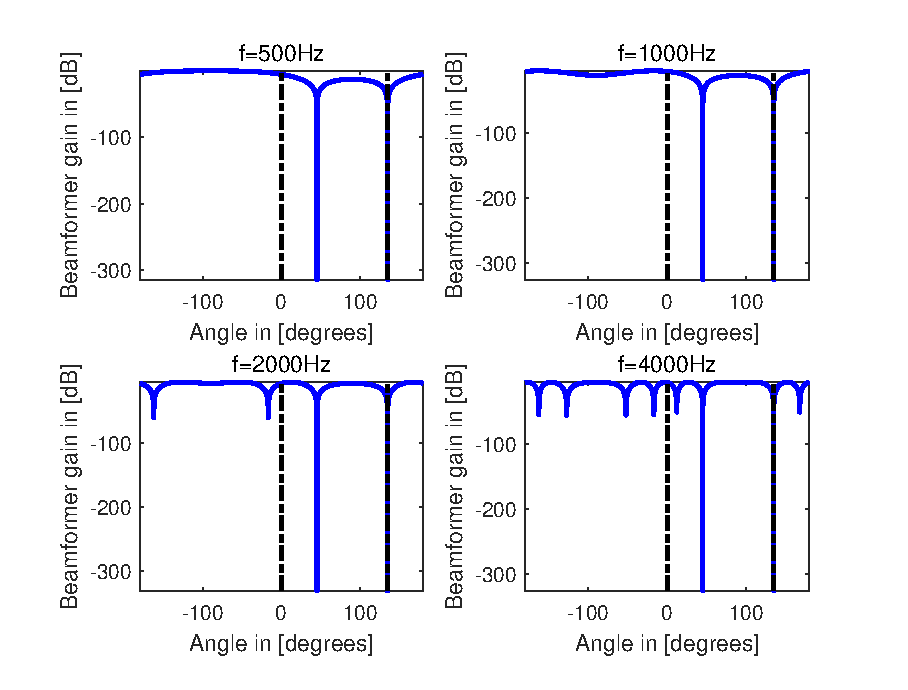
\includegraphics[width=1\textwidth]{img/1_a_2.eps}}
	\caption{Beampattern of upper two microphones}
	\label{Beampattern of upper two microphones135}
\end{minipage}
	\hfill
\begin{minipage}[b]{0.5\linewidth}
	\centerline{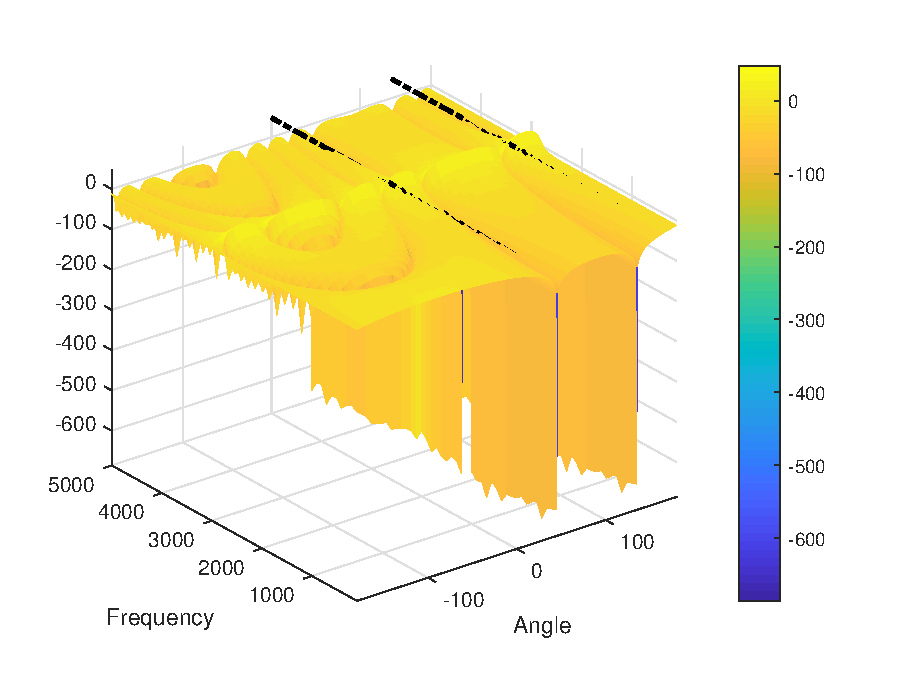
\includegraphics[width=1\textwidth]{img/1_a_2_multi_135.eps}}
	\caption{Multitone beampattern of upper two microphones}
	\label{Multitone beampattern of upper two microphones135}
\end{minipage}
\end{figure}

\begin{figure}[htbp]
	\begin{minipage}[b]{0.5\linewidth}
		\centerline{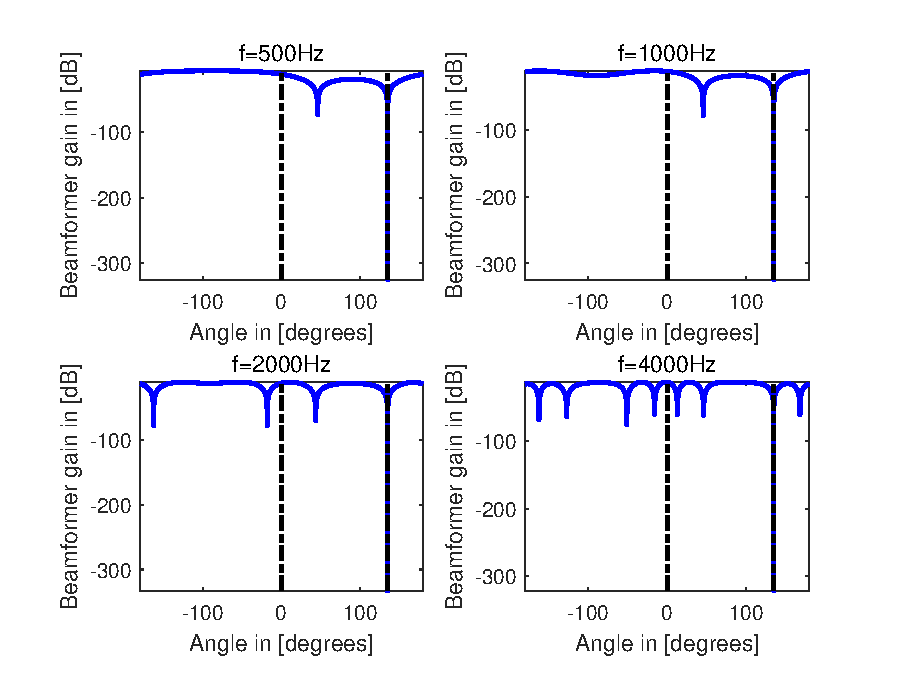
\includegraphics[width=1\textwidth]{img/1_a_3.eps}}
		\caption{Beampattern of all four microphones}
		\label{Beampattern of all four microphones135}
	\end{minipage}
	\hfill
	\begin{minipage}[b]{0.5\linewidth}
		\centerline{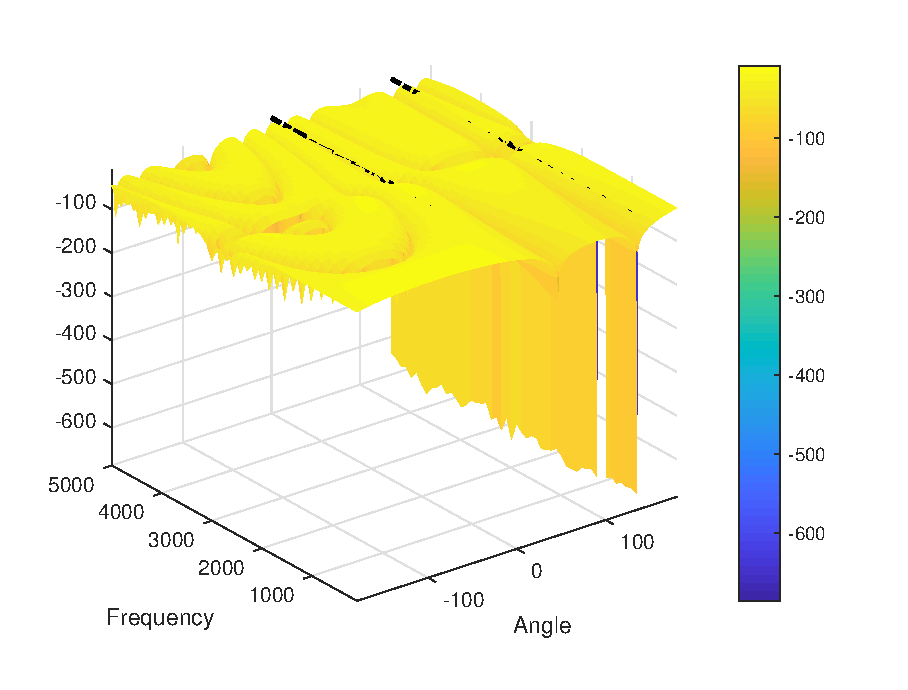
\includegraphics[width=1\textwidth]{img/1_a_3_multi_135.eps}}
		\caption{Multitone beampattern of all four microphones}
		\label{Multitone beampattern of all four microphones135}
	\end{minipage}
\end{figure}




\subsection{Desired source located at 0 degrees and Interferer located at 45 degrees}

When the interferer is located at \(45^{\circ}\) instead of \(135^{\circ}\), the beampatterns change correspondingly. When we use the upper two microphones, the results are almost the same as an \(135^{\circ}\) interferer, that's because the symmetry we mentioned before.



\begin{figure}[htbp]
	\begin{minipage}[b]{0.5\linewidth}
		\centerline{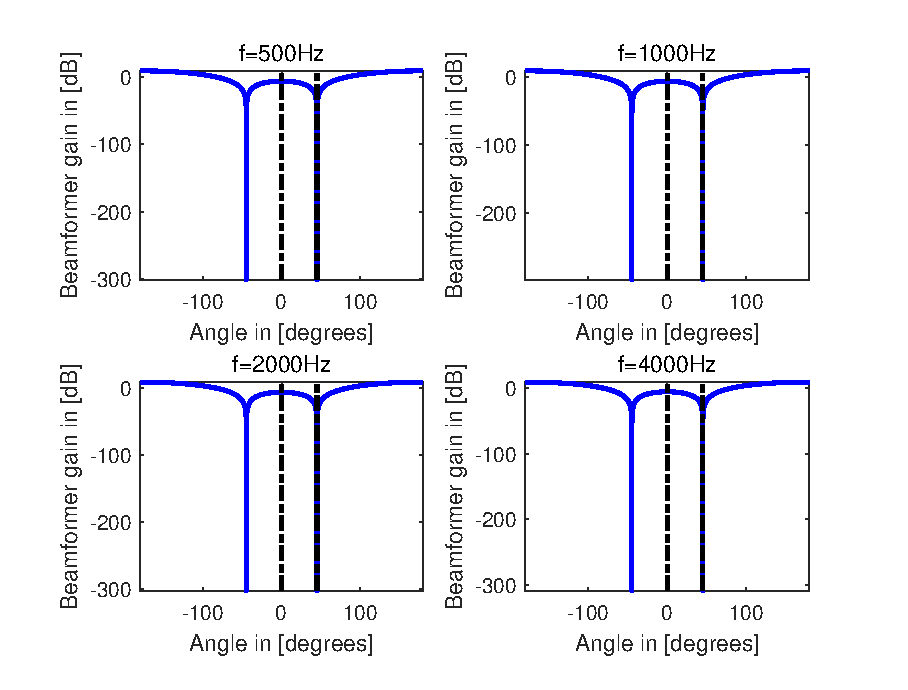
\includegraphics[width=1\textwidth]{img/1_b_1.eps}}
		\caption{Beampattern of left two microphones}
		\label{Beampattern of left two microphones45}
	\end{minipage}
	\hfill
	\begin{minipage}[b]{0.5\linewidth}
		\centerline{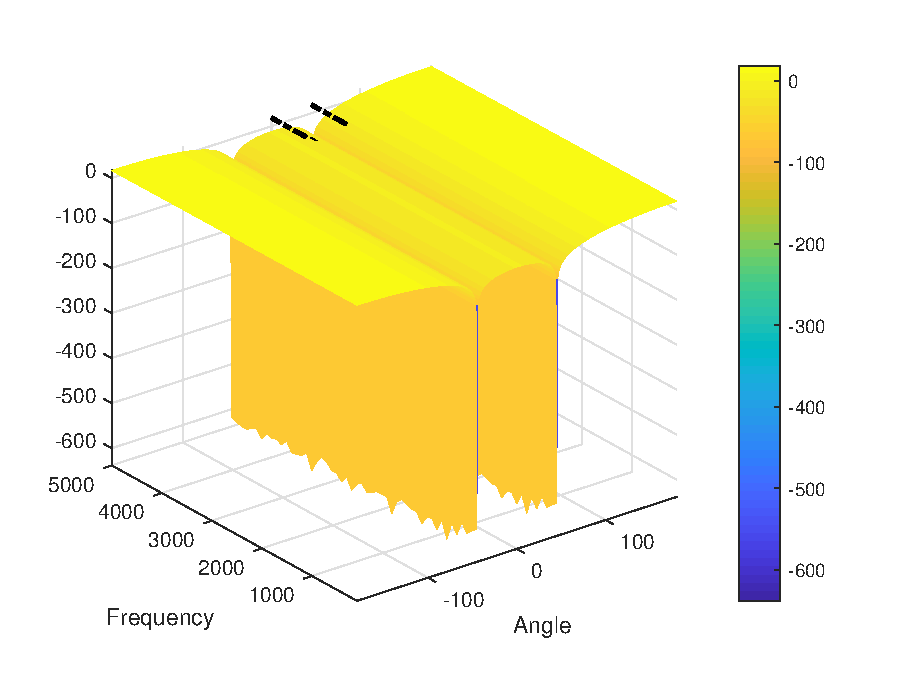
\includegraphics[width=1\textwidth]{img/1_a_1_multi_45.eps}}
		\caption{Multitone beampattern of left two microphones}
		\label{Multitone beampattern of left two microphones45}
	\end{minipage}
\end{figure}

\begin{figure}[htbp]
	\begin{minipage}[b]{0.5\linewidth}
		\centerline{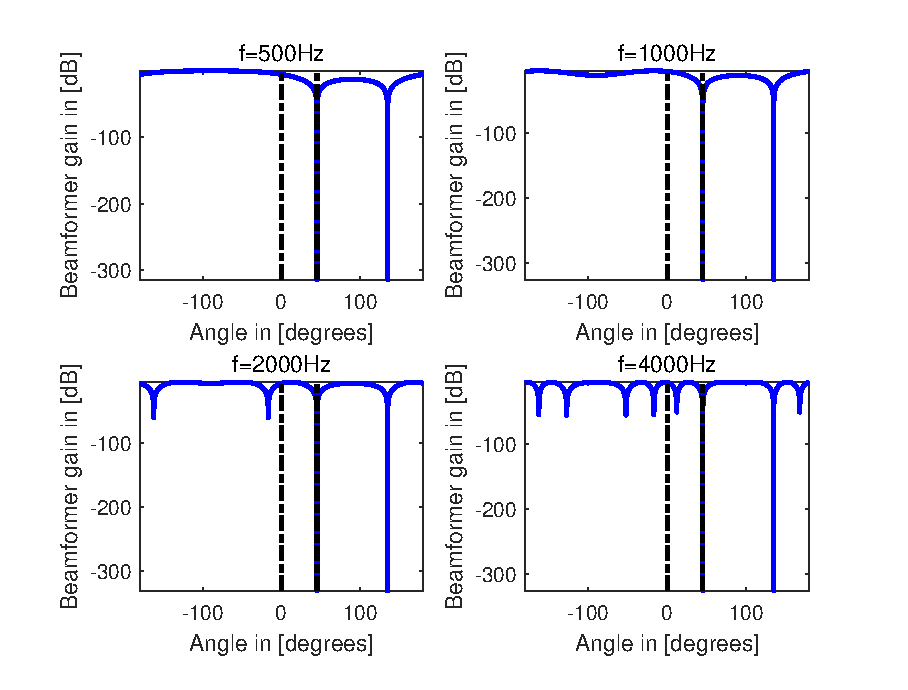
\includegraphics[width=1\textwidth]{img/1_b_2.eps}}
		\caption{Beampattern of upper two microphones}
		\label{Beampattern of upper two microphones45}
	\end{minipage}
	\hfill
	\begin{minipage}[b]{0.5\linewidth}
		\centerline{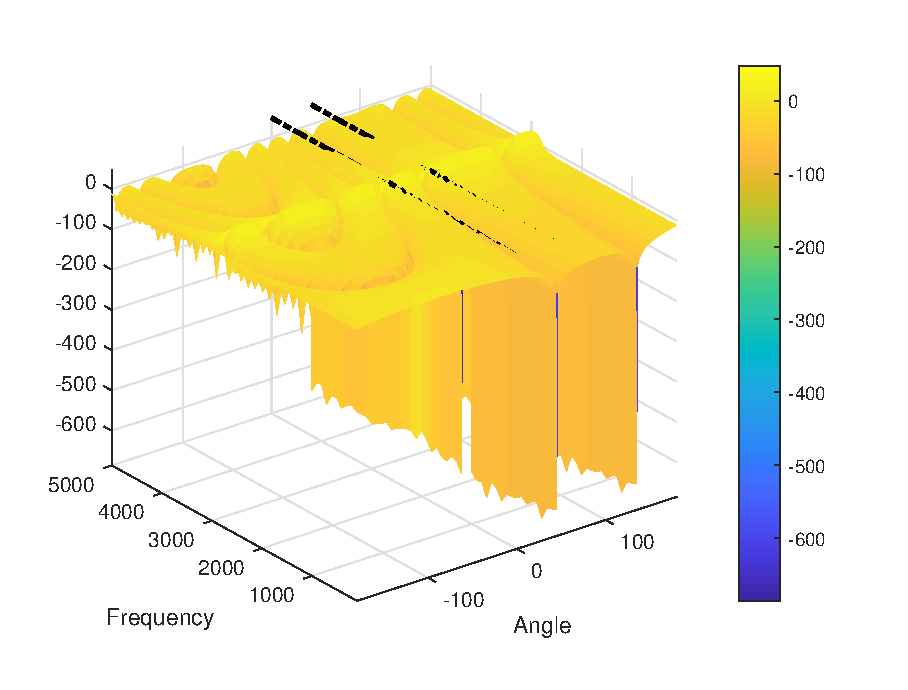
\includegraphics[width=1\textwidth]{img/1_a_2_multi_45.eps}}
		\caption{Multitone beampattern of upper two microphones}
		\label{Multitone beampattern of upper two microphones45}
	\end{minipage}
\end{figure}

\begin{figure}[htbp]
	\begin{minipage}[b]{0.5\linewidth}
		\centerline{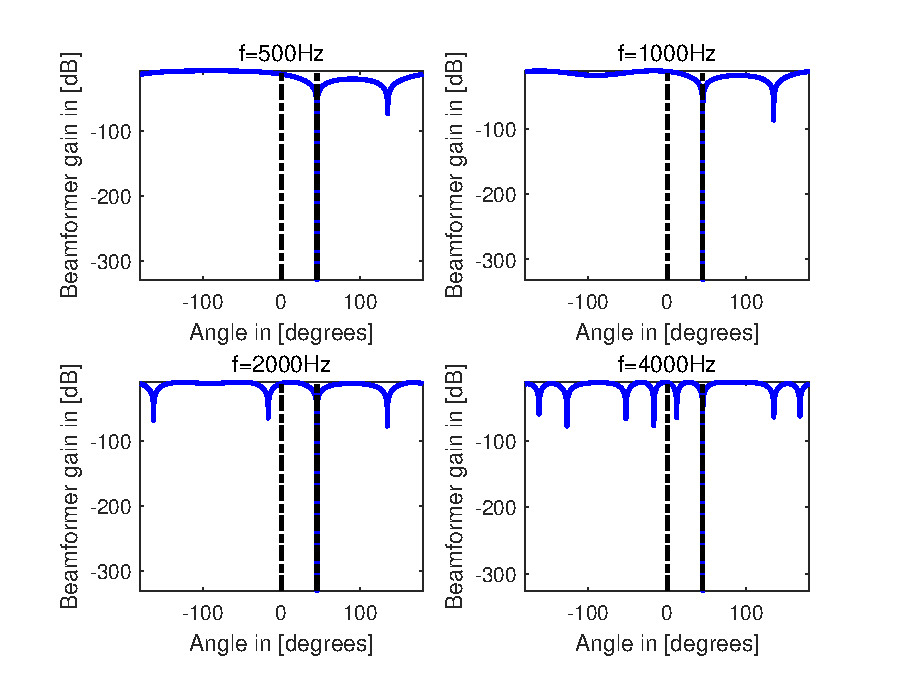
\includegraphics[width=1\textwidth]{img/1_b_3.eps}}
		\caption{Beampattern of all four microphones}
		\label{Beampattern of all four microphones45}
	\end{minipage}
	\hfill
	\begin{minipage}[b]{0.5\linewidth}
		\centerline{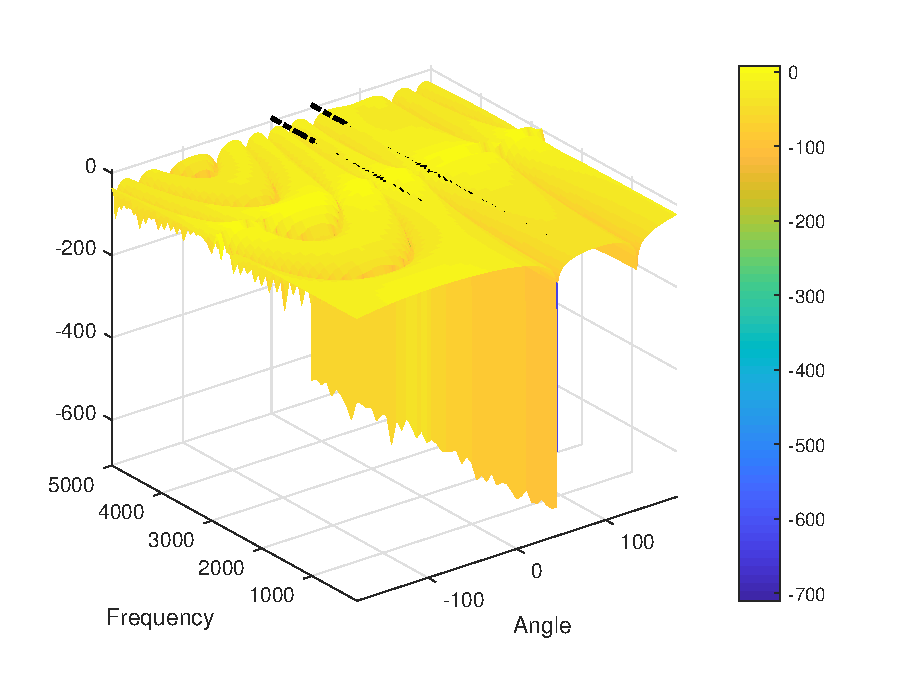
\includegraphics[width=1\textwidth]{img/1_a_3_multi_45.eps}}
		\caption{Multitone beampattern of all four microphones}
		\label{Multitone beampattern of all four microphones45}
	\end{minipage}
\end{figure}

\section{Fractional delay}

\subsection{Inverse Fourier transform}

\begin{equation}
\begin{aligned}
d[n]&= \frac{1}{2\pi}\int_{-\pi}^{\pi}D(e^{j\theta})e^{jn\theta}d\theta \\
 &= \frac{1}{2\pi}\int_{-\pi}^{\pi}e^{j(n-\tau)\theta}d\theta \\
 &= \frac{1}{2\pi} \frac{1}{j(n-\tau)} e^{j(n-\tau)\theta} \Big|_{-\pi}^{\pi} \\
 &= \frac{e^{j(n-\tau)\pi}-e^{-j(n-\tau)\pi}}{2\pi j(n-\tau)} \\ 
 &= \frac{2j\sin((n-\tau)\pi)}{2\pi j(n-\tau)} \\
 &= \rm{sinc}(n-\tau)
\end{aligned}
\label{eq}
\end{equation}

\subsection{Figure of analytical expressions of the impulse responses}

Fig.\ref{Analytical values of the impulse responses} shows theoretical values of the impulse responses.

\begin{figure}[htbp]
	\centerline{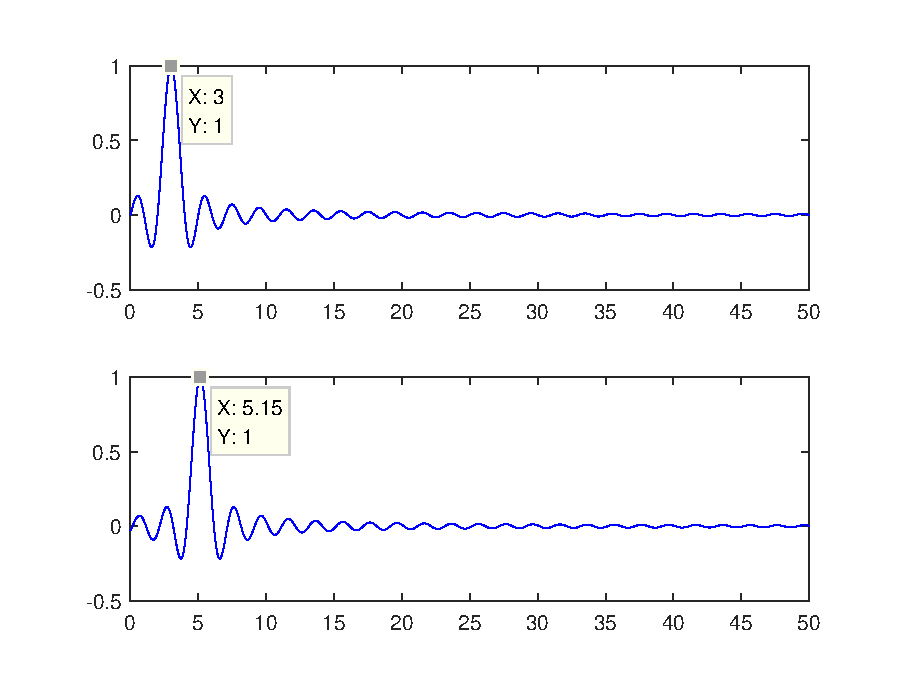
\includegraphics[width=0.65\textwidth]{img/2_b_2.eps}}
	\caption{Analytical values of the impulse responses (upper:\(\tau \)=3 lower:\(\tau \)=5.15)}
	\label{Analytical values of the impulse responses}
\end{figure}

\subsection{Figure of the impulse responses}

From the result of Fig.~\ref{Values of the impulse responses}, we find out that the stem plot of \textbf{delay.m} program is delayed version theoretical \textbf{sinc} function. Therefore, if we want to use \textbf{h = delay(d, fd, L, dmax)} to delay one of the sensor channels, we have to be careful with the unusual delay to prevent noncausality. One of the solutions is to circularshift it back to where it ought to be. In our project, we use another solution in the following parts, which is giving lower two sensor channels a \textbf{h = delay(0, 0, L, 1)} convolution. This makes all the channels time-aligned by giving all of them a same unusual delay. So, the causality is preserved.

\begin{figure}[htbp]
	\centerline{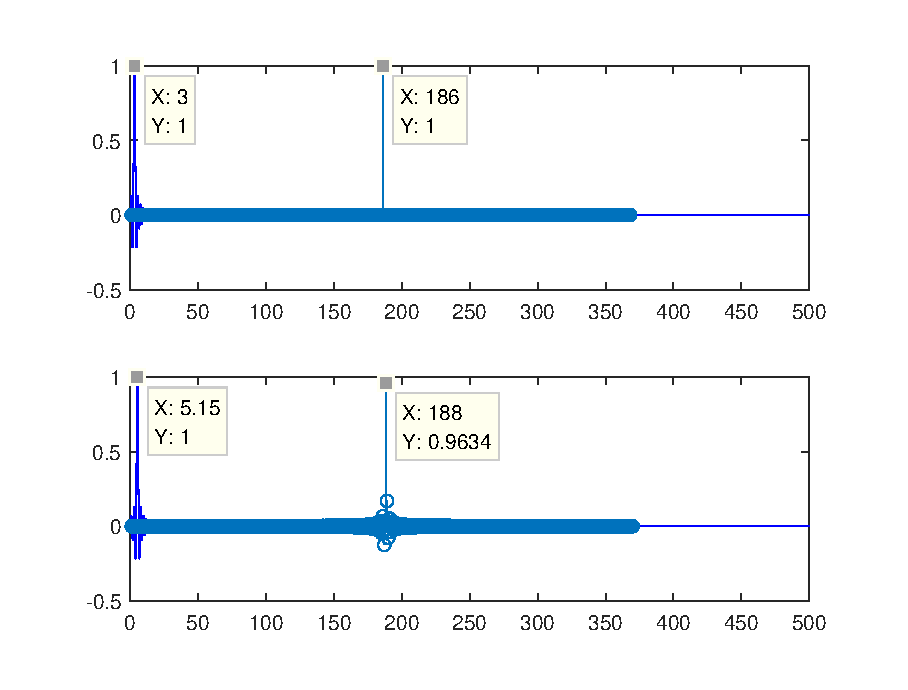
\includegraphics[width=0.65\textwidth]{img/2_b_3.eps}}
	\caption{Values of the impulse responses (upper:\(\tau \)=3 lower:\(\tau \)=5.15)}
	\label{Values of the impulse responses}
\end{figure}

\section{Scenario 2: GSC applied to monaural hearing aid}\label{monaural}

\subsection{Delay and sum beamformer results}

We can hear a speech consisting of desired source, interference and background noise, $v_0$ is noise-reduced. The delay of the upper sensor $x_1$ is calculated as 
\begin{equation*}
	\text{delay} = \frac{dy}{c}\cdot f_s =\frac{0.01}{340} \times 8000 \doteq 0.235 \text{s}
\end{equation*}
Because this delay is too small, human ears can not distinguish the difference between signals before and after delay. The result is that the desired signals become time-aligned in each sensor, while interference and noise are not. 
\subsection{Blocking matrix effect}

After a delay-beamformer, the desired signals are time-aligned. We use blocking matrix B=[-1,1], to eliminate these time-aligned signals and thus get interference and background noise that are not time-aligned.

You can verify the signal after blocking matrix operation through the audio ``\textit{block desired source.wav}''.
\subsection{Adaptive filter algorithm}

Fig.~\ref{NLMS adaptive filter coefficient with left two sensors} and Fig.~\ref{RLS adaptive filter coefficient with left two sensors} are the filter coefficient of NLMS and RLS. It's hard to tell the difference of the result audios using these algorithms, as they both reduce noise to some extent. Since RLS has faster convergence, we choose RLS when using the left two sensors.

\begin{figure}[htbp]
	\begin{minipage}[b]{0.5\linewidth}
	\centerline{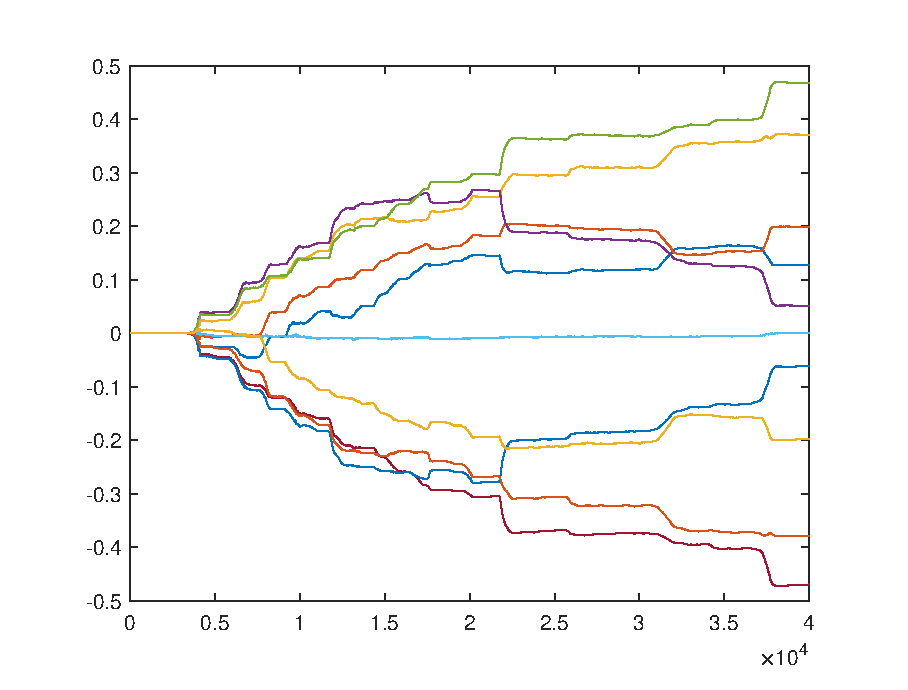
\includegraphics[width=1\textwidth]{img/NLMS_2sensor.eps}}
	\caption{NLMS adaptive filter coefficient with left two sensors}
	\label{NLMS adaptive filter coefficient with left two sensors}
	\end{minipage}
	\hfill
	\begin{minipage}[b]{0.5\linewidth}
	\centerline{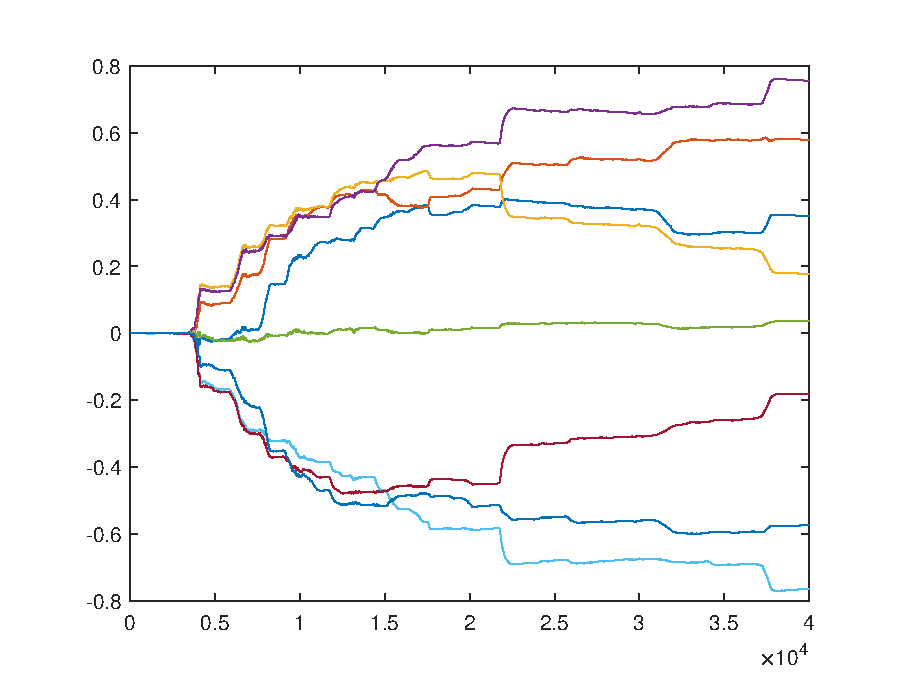
\includegraphics[width=1\textwidth]{img/RLS_2sensor.eps}}
	\caption{RLS adaptive filter coefficient with left two sensors}
	\label{RLS adaptive filter coefficient with left two sensors}
	\end{minipage}
\end{figure}

\subsection{Transfer function and multitone	beampattern comparision}
Note that we do not use $\Delta$ to give delay, but solve the time alignment by other ways.

\begin{equation}
\begin{aligned}
Y&= \frac{1}{2}(X_1H_1+X_2H_2)-(X_2H_2-X_1H_1)W \\
&=(\frac{1}{2}+W)H_1X_1+(\frac{1}{2}-W)H_2X_2
\end{aligned}
\label{eq}
\end{equation}

Substitute in \(H_1=e^{-j(\tau+\frac{0.01}{340})\theta} \) and \(H_2=e^{-j\tau\theta}\) we can get the transfer function:

\begin{equation}
\frac{Y}{X_1}=(\frac{1}{2}+W)H_1 = (\frac{1}{2}+W)e^{-j(\tau+\frac{0.01}{340})\theta}
\label{eq}
\end{equation}

\begin{equation}
\frac{Y}{X_2}=(\frac{1}{2}-W)H_2 = (\frac{1}{2}-W)e^{-j\tau\theta}
\label{eq}
\end{equation}

Fig.~\ref{Multitone beampattern with left two sensors (without beam-steering)} is different with Fig.~\ref{Multitone beampattern of left two microphones135} and Fig.~\ref{Multitone beampattern of left two microphones45} because Fig.~\ref{Multitone beampattern with left two sensors (without beam-steering)} is the multitone beampattern without beamsteering. It is the inherent property of array. We can see the peaks at $+90^{\circ}$ and $-90^{\circ}$, and valley at $0^{\circ}$ in Fig.~\ref{Multitone beampattern with left two sensors (without beam-steering)}.

\begin{figure}[htbp]
	\centerline{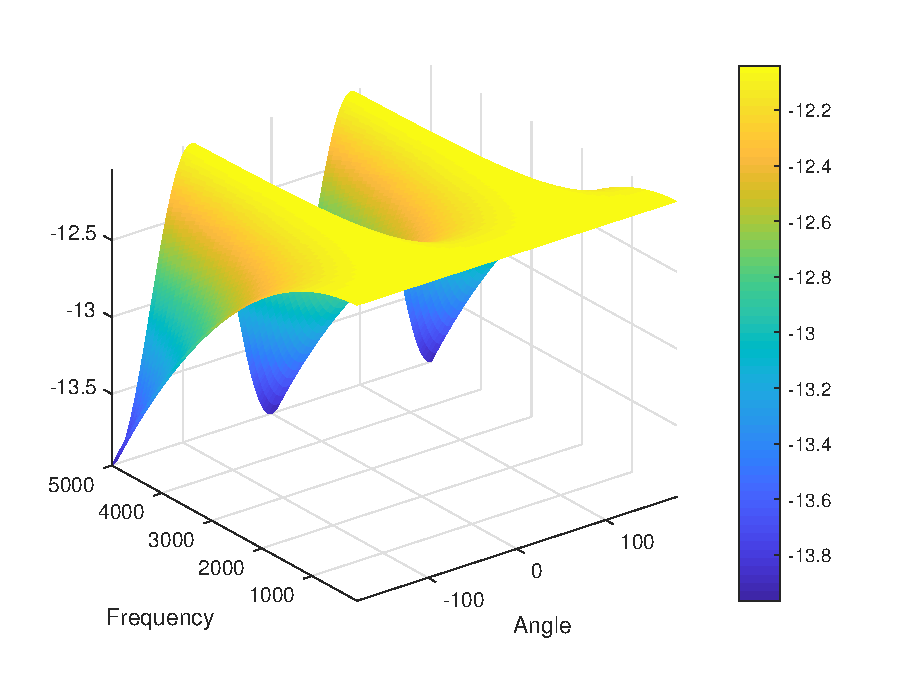
\includegraphics[width=0.5\textwidth]{img/multi_left2.eps}}
	\caption{Multitone beampattern with left two sensors (without beam-steering)}
	\label{Multitone beampattern with left two sensors (without beam-steering)}
\end{figure}
\begin{figure}[htbp]
	\centerline{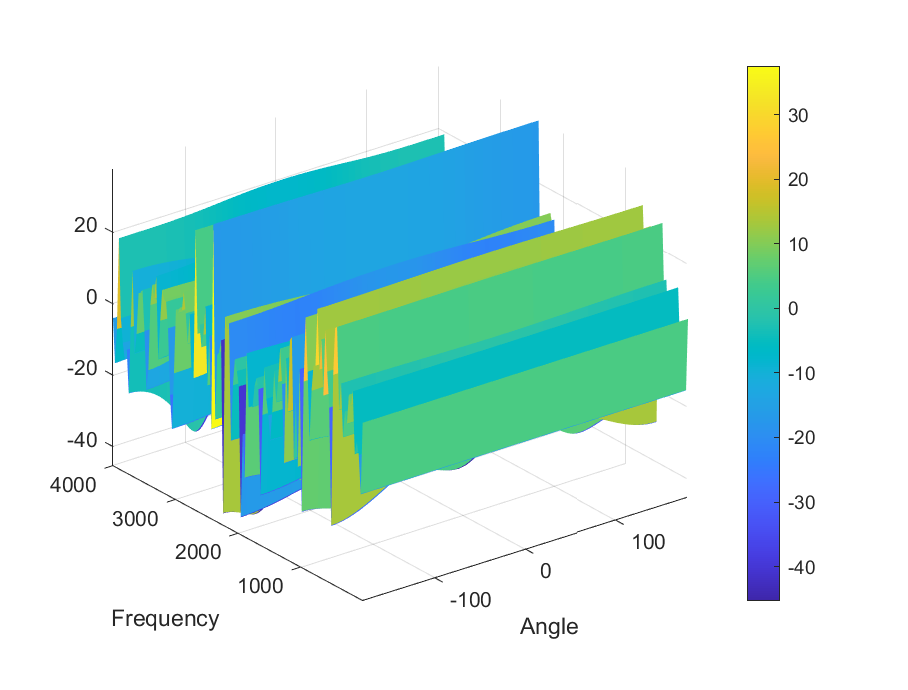
\includegraphics[width=0.5\textwidth]{img/trans_NMLS_2sensor.eps}}
	\caption{Beampattern of the array weighted by transfer function calculated by NLMS data (2 sensors)}
	\label{Transfer function calculated by NLMS data}
\end{figure}
\begin{figure}[htbp]
	\centerline{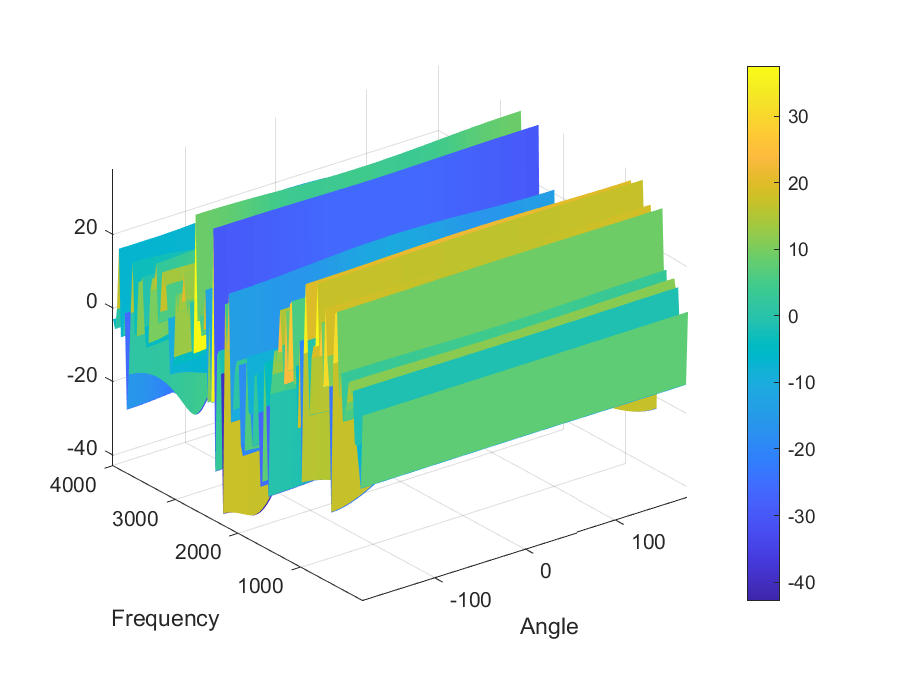
\includegraphics[width=0.5\textwidth]{img/trans_RLS_2sensor.eps}}
	\caption{Beampattern of the array weighted by transfer function calculated by RLS data (2 sensors)}
	\label{Transfer function calculated by RLS data (2 sensors)}
\end{figure}

Fig.~\ref{Transfer function calculated by NLMS data} and Fig.~\ref{Transfer function calculated by RLS data (2 sensors)} are the beampatterns of the array weighted by transfer functions calculated by input and output data in frequency domain.
\section{Scenario 3: GSC applied to binaural hearing aids}

\subsection{Delay and sum beamformer results}

We can hear a speech consisting of desired source, interference and background noise, $v_0$ is noise-reduced. The delay of the both upper sensors $x_1$ and $x_4$ is calculated the same way in Sec. \ref{monaural}.
\begin{equation*}
\text{delay} = \frac{dy}{c}\cdot f_s =\frac{0.01}{340} \times 8000 \doteq 0.235 \text{s}
\end{equation*}
Because this delay is too small, human ears can not distinguish the difference between signals before and after delay. The result is that the desired signals become time-aligned in each sensor, while interference and noise are not. 

\subsection{Blocking matrix effect}

\begin{equation}       
B = \begin{bmatrix}
-1 & 1 & 0 & 0\\ 
-1 & 0 & 1 & 0\\  
-1 & 0 & 0 & 1
\end{bmatrix}     
\end{equation}
We use blocking matrix B, to eliminate these time-aligned signals and thus get interference and background noise that are not time-aligned.

You can verify the signals after blocking matrix operation through the audios ``\textit{block desired source 4 sensor\_1.wav}'', ``\textit{block desired source 4 sensor\_2.wav}'' and ``\textit{block desired source 4 sensor\_3.wav}''.
\subsection{Adaptive filter algorithm}
Fig.~\ref{FDAF coeff} and Fig.~\ref{RLS coeff} are the filter coefficients of FDAF and RLS. They all converge to some values, but FDAF is faster-convergent and stabler than RLS. As for the result audios, FDAF eliminates the interference better but not the noise, While RLS reduces noise but has hardly any elimination on interference.

\begin{figure}[htbp]
	\centering
	\subfigure[channel 1]{
		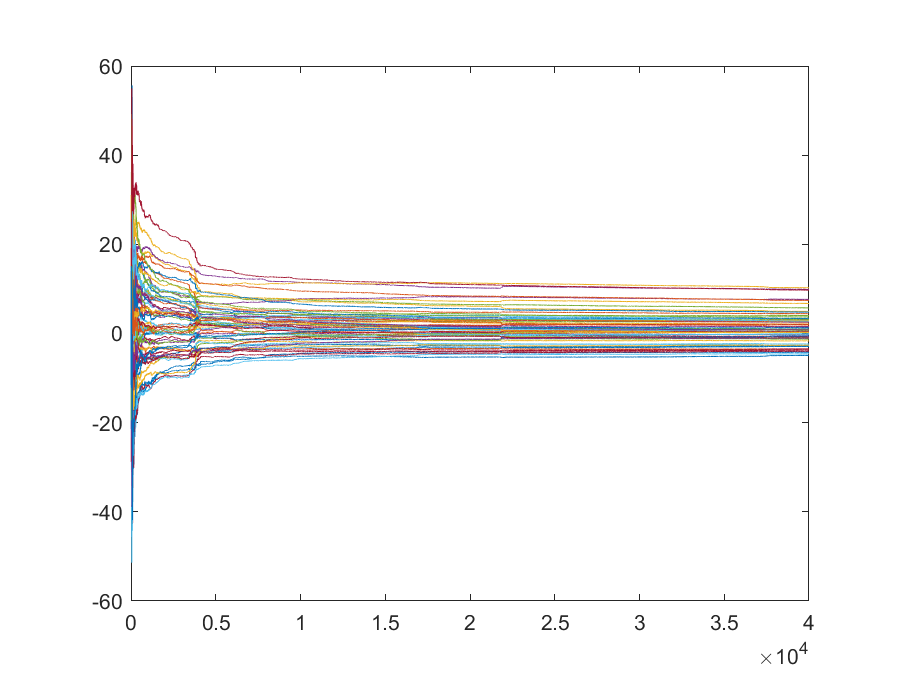
\includegraphics[width=0.3\textwidth]{img/FDAF_4sensor_1.eps}
	}\label{FDAF coeff 1}
	\quad
	\subfigure[channel 2]{
		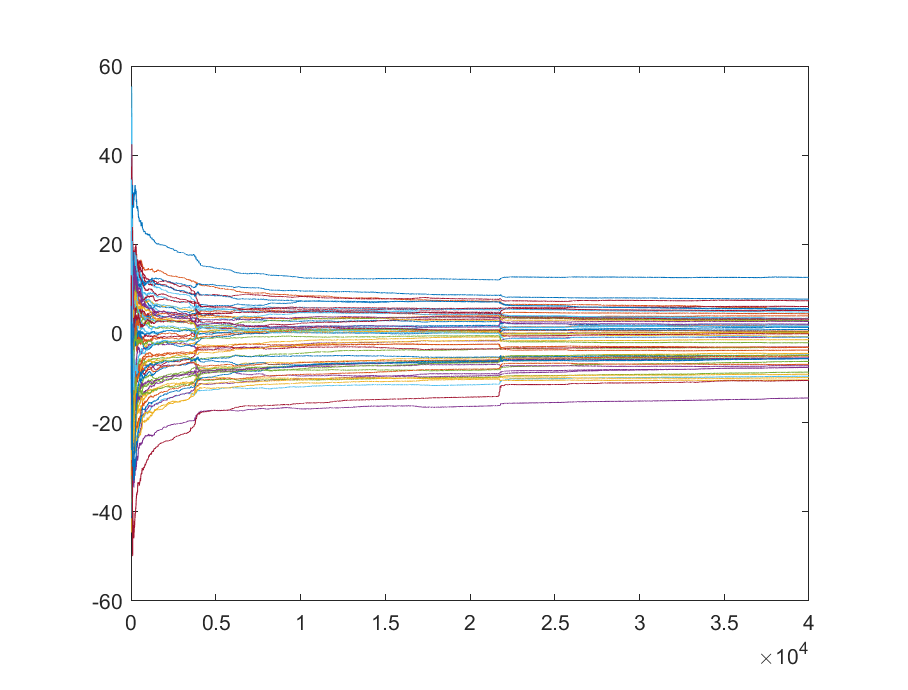
\includegraphics[width=0.3\textwidth]{img/FDAF_4sensor_2.eps}
	}\label{FDAF coeff 2}
	\quad
	\subfigure[channel 3]{
		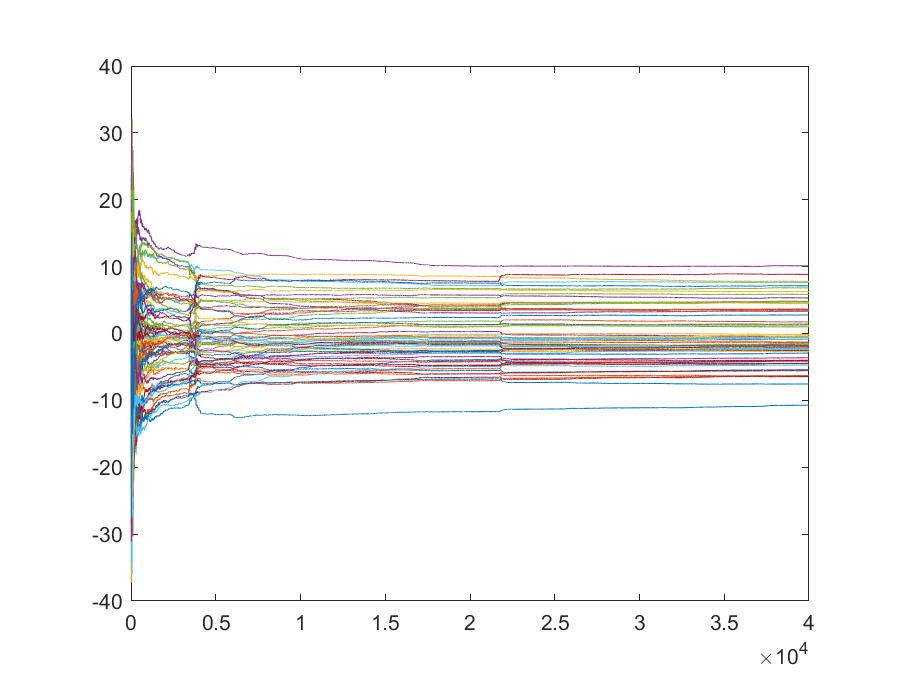
\includegraphics[width=0.3\textwidth]{img/FDAF_4sensor_3.eps}
	}\label{FDAF coeff 3}
		\caption{FDAF adaptive filter coefficient with all four sensors}\label{FDAF coeff}
\end{figure}

\begin{figure}[htbp]
	\centering
	\subfigure[channel 1]{
		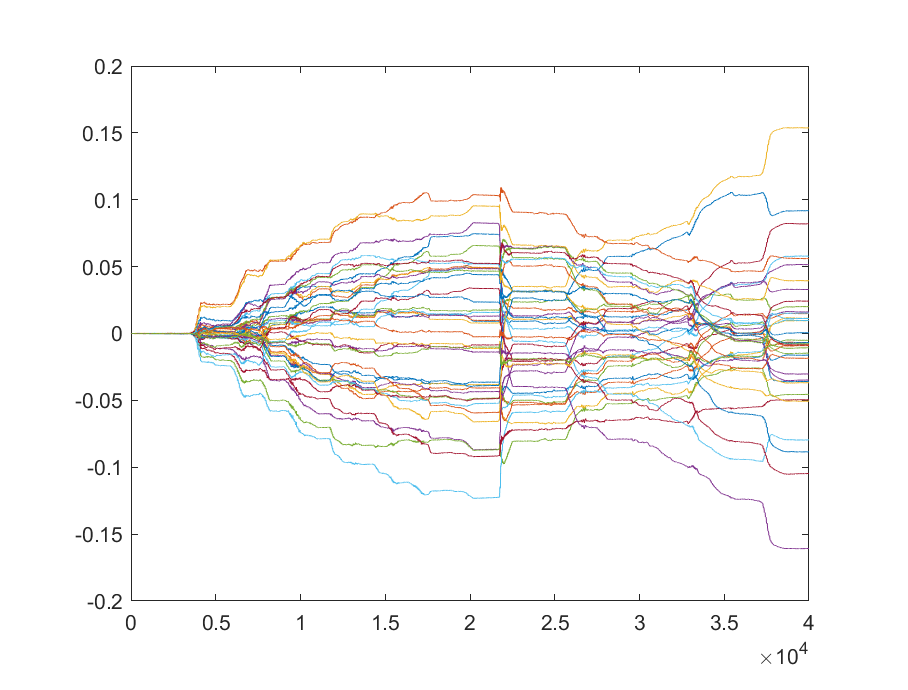
\includegraphics[width=0.3\textwidth]{img/RLS_4sensor_1.eps}
	}\label{RLS coeff 1}
	\quad
	\subfigure[channel 2]{
		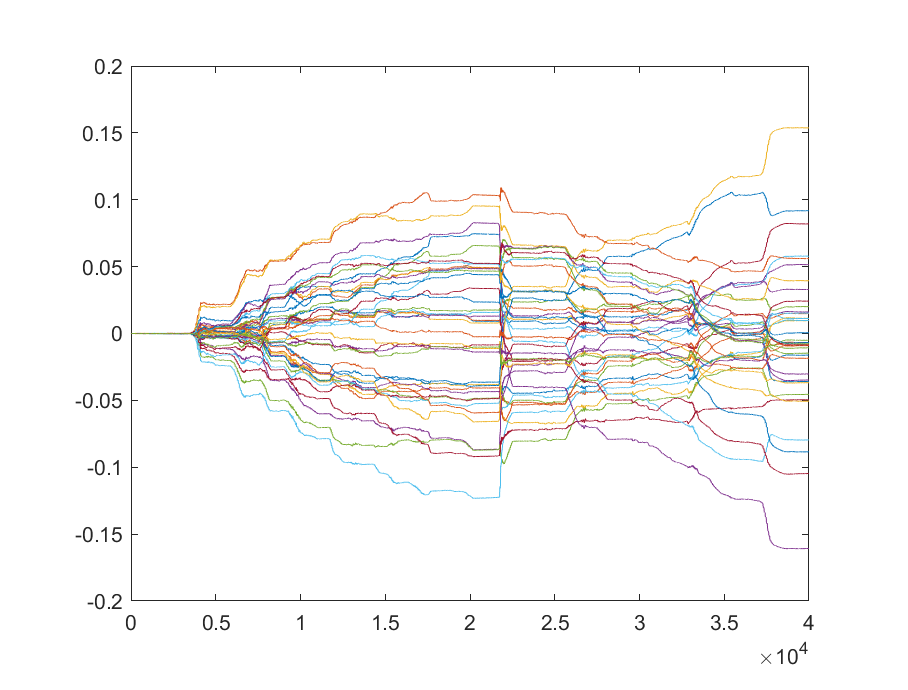
\includegraphics[width=0.3\textwidth]{img/RLS_4sensor_2.eps}
	}\label{RLS coeff 2}
	\quad
	\subfigure[channel 3]{
		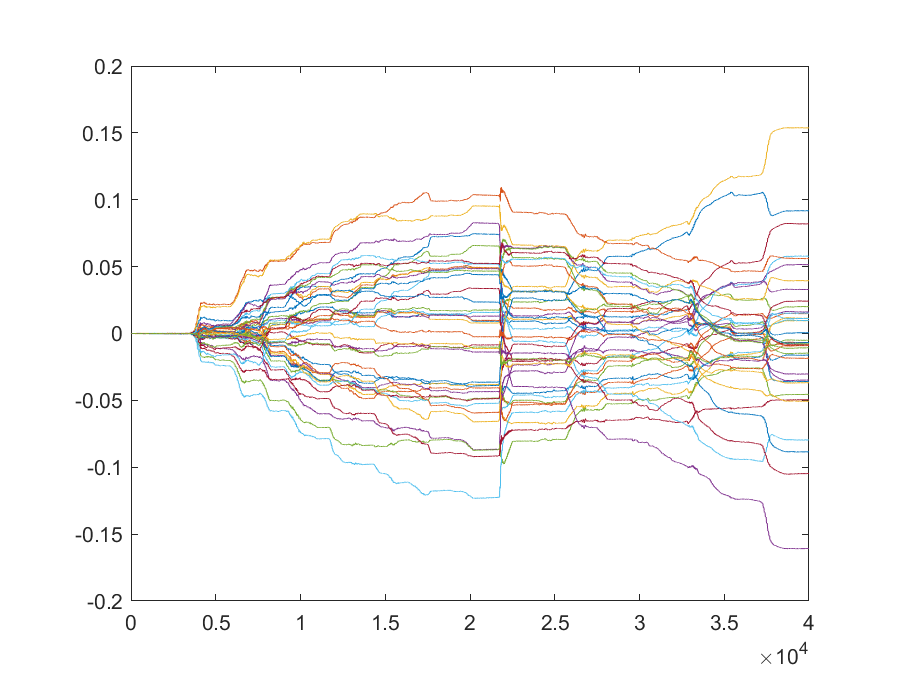
\includegraphics[width=0.3\textwidth]{img/RLS_4sensor_3.eps}
	}\label{RLS coeff 3}
	\caption{RLS adaptive filter coefficient with all four sensors}\label{RLS coeff}
\end{figure}
\subsection{Transfer function and multitone	beampattern comparision}
Note that we do not use $\Delta$ to give delay, but solve the time alignment by other ways.

\begin{equation}
Y= \frac{1}{4}(X_1H_1+X_2H_2+X_3H_2+X_4H_1)-\frac{1}{3}[(X_2H_2-X_1H_1)W_1+(X_3H_2-X_1H_1)W_2+(X_4H_1-X_1H_1)W_3] 
\label{eq}
\end{equation}

Substitute in \(H_1=e^{-j(\tau+\frac{0.01}{340})\theta} \) and \(H_2=e^{-j\tau\theta}\) we can get the transfer function:

\begin{equation}
\begin{aligned}
\frac{Y}{X_1}&=\frac{1}{4}H_1+\frac{1}{3}H_1W_1+\frac{1}{3}H_1W_2+\frac{1}{3}H_1W_3 
=[\frac{1}{4}+\frac{1}{3}(W_1+W_2+W_3)]H_1 \\   &= [\frac{1}{4}+\frac{1}{3}(W_1+W_2+W_3)]e^{-j(\tau+\frac{0.01}{340})\theta}
\end{aligned}
\label{eq}
\end{equation}

\begin{equation}
\begin{aligned}
\frac{Y}{X_2}&=\frac{1}{4}H_2-\frac{1}{3}H_2W_1
=(\frac{1}{4}-\frac{1}{3}W_1)H_2 \\   &= (\frac{1}{4}-\frac{1}{3}W_1)e^{-j\tau\theta}
\end{aligned}
\label{eq}
\end{equation}

\begin{equation}
\begin{aligned}
\frac{Y}{X_3}&=\frac{1}{4}H_2-\frac{1}{3}H_2W_2
=(\frac{1}{4}-\frac{1}{3}W_2)H_2 \\   &= (\frac{1}{4}-\frac{1}{3}W_2)e^{-j\tau\theta}
\end{aligned}
\label{eq}
\end{equation}

\begin{equation}
\begin{aligned}
\frac{Y}{X_4}&=\frac{1}{4}H_1-\frac{1}{3}H_1W_3
=(\frac{1}{4}-\frac{1}{3}W_3)H_1 \\   &= (\frac{1}{4}-\frac{1}{3}W_3)e^{-j(\tau+\frac{0.01}{340})\theta}
\end{aligned}
\label{eq}
\end{equation}

Fig.~\ref{Multitone beampattern with all 4 sensors} is different with Fig.~\ref{Multitone beampattern of all four microphones135} and Fig.~\ref{Multitone beampattern of all four microphones45} because Fig.~\ref{Multitone beampattern with all 4 sensors} is the multitone beampattern without beamsteering. It is the inherent property of array.

\begin{figure}[htbp]
	\centerline{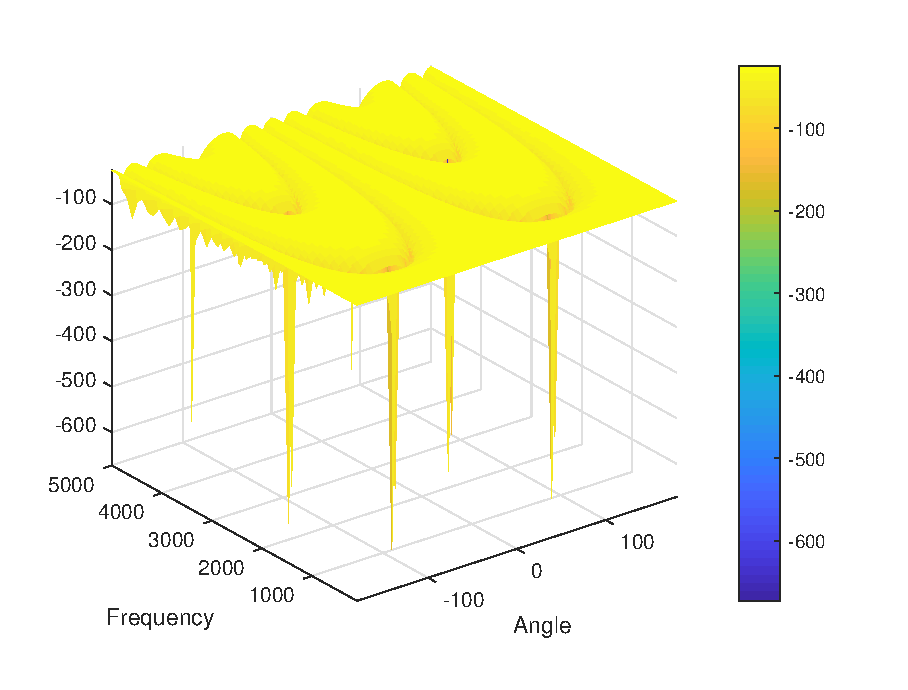
\includegraphics[width=0.5\textwidth]{img/multi_all4.eps}}
	\caption{Multitone beampattern with all 4 sensors}
	\label{Multitone beampattern with all 4 sensors}
\end{figure}

Fig.~\ref{Transfer function calculated by FDAF data} and Fig.~\ref{Transfer function calculated by RLS data (4 sensors)} are the beampatterns of the array weighted by transfer functions calculated by input and output data in frequency domain.
\begin{figure}[htbp]
	\centerline{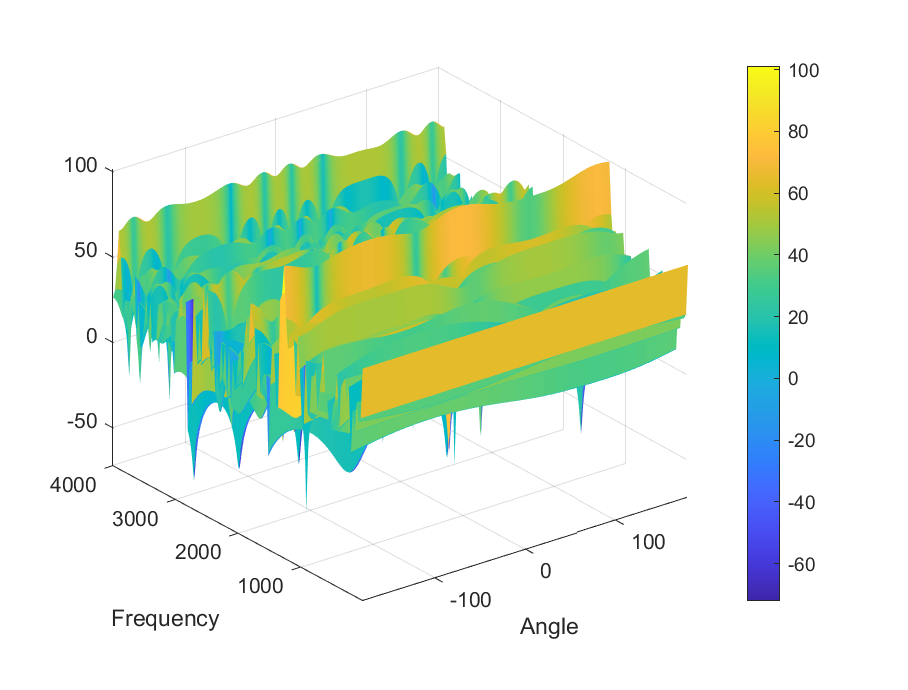
\includegraphics[width=0.5\textwidth]{img/trans_FDAF_4sensor.eps}}
	\caption{Beampattern of the array weighted by transfer function calculated by FDAF data (4 sensors)}
	\label{Transfer function calculated by FDAF data}
\end{figure}
\begin{figure}[htbp]
	\centerline{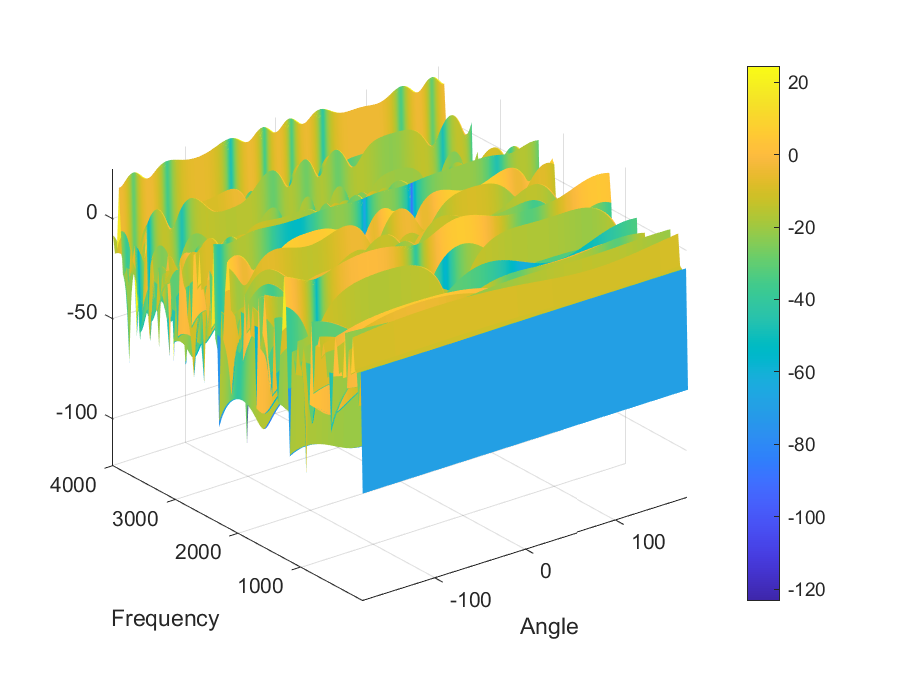
\includegraphics[width=0.5\textwidth]{img/trans_RLS_4sensor.eps}}
	\caption{Beampattern of the array weighted by transfer function calculated by RLS data (4 sensors)}
	\label{Transfer function calculated by RLS data (4 sensors)}
\end{figure}












\end{document}
